\documentclass{article}
\usepackage{fullpage}
\usepackage{parskip}
\usepackage[usenames,dvipsnames,svgnames,table]{xcolor} % Provides more color options
\usepackage[bookmarks,colorlinks,linktoc=all,linkcolor=DarkGreen,urlcolor=Blue]{hyperref}
\usepackage{graphicx}
\usepackage[symbol]{footmisc}
\title{Proposal for the Implementation of an Laser Shooting Range}
\author{Matt Kline, James Gordon, Tyler Kuske, and Creighton Long}
\begin{document}
\maketitle
\newpage
\tableofcontents
\newpage

\section{Executive Summary}

The proposed project is a virtual shooting range.
The setup will consist of multiple targets which can be placed around a room.
Each target would consist of a laser receiver as well as some LEDs, and will be connected to our ZedBoard via radio link.

Multiple players would then have a laser emitting ``gun''
consisting of (at minimum) a processor package, a laser, a speaker, and a wireless transmitter.
Each gun would be configured to emit a unique laser sequence when the trigger is pulled,
which the ZedBoard/target setup would use to determine which player hit a target.
Further work is mostly software-based with several games and scenarios,
such as timing drills or hitting multiple targets in a sequence, could be played with one or more players.
Statistics will be tracked by the ZedBoard and can be displayed using a desktop or mobile application.

\newpage

\section{Detailed Report}

\subsection{Objectives}

\subsubsection{Primary}

The following goals should be considered basic benchmarks for the project.

\begin{itemize}
\item At least two laser ``guns'', each able to emit their own unique laser signature, sound, and wireless signal
\item At least three target modules with laser receivers and LEDs
\item At least one single player game/drill
\item At least one multiplayer game/drill
\item Statistic tracking via the ZedBoard
\item Statistic display and game controls via a desktop or mobile application
\end{itemize}

\subsubsection{Secondary Goals}

The following goals are additional features to be developed once the primary goals are met.

\begin{itemize}
\item Additional targets
\item Pop-up or moving targets
\item Force feedback on the ``guns'' to simulate recoil
\item Additional game modes and statistics
\item Ability to track stability while aiming (likely through the use of an accelerometer)
\end{itemize}

\subsection{Design Plan}

\subsubsection{Hardware}

\paragraph{Guns}

Each gun will consist of
\begin{itemize}
\item A laser diode
\item A collimating lens to focus the laser into a tight beam
\item A small speaker for user feedback
\item A multicolor LED for indicating status to the player (If design space and I/O pins permit)
\item A TI CC430 for logic and radio communications
\item An accelerometer for tracking the steadiness of the shooter before pulling the trigger.
\item A supporting PCB
\end{itemize}

All of the gun's hardware will be enclosed in a gun-shaped controller with some sort of trigger mechanism.
A Namco GunCon or similar is suggested as it should have ample room for housing the parts as well as a built-in trigger.

\paragraph{Targets}

Each target will consist of
\begin{itemize}
\item One or more phototransistors to detect incoming laser signals from the guns
\item A series of multicolor LEDs for prompting a player to shoot at the target
\item A small speaker for user feedback
\item A TICC430 for logic and radio communications
\item A supporting PCB
\end{itemize}

\paragraph{Central Control}

The daughter card for the ZedBoard will consist of a TICC430 that will do minor processing and route communications
back to the ZedBoard, and any needed accompanying hardware.
The ZedBoard will manage the peripherals, handle game logic, and update the UI.
The ZedBoard's FPGA, at the instructor's suggestion, can be used to handle the board's switches and display.

\subsubsection{Software}

\paragraph{Guns}

The gun's software will run on the CC430 and accomplish the following tasks:
\begin{itemize}
\item Use the laser diode to emit a unique laser sequence when the trigger is pulled.
	This will be used to uniquely identify each gun.
\item Provide audio feedback when the trigger is pulled, and perhaps when the game starts/ends.
\item Provide visual feedback via the LED indicating the player's color, game status, etc.
\item Maintain a circular buffer of accelerometer information and take a snapshot when the trigger is pulled.
	This will provide information about the user's stability up to his trigger squeeze.
\item Respond to radio communication when needed.
\end{itemize}

To keep comms down, and since the guns themselves do not require any immediate response from the rest of the system
when the game is being played, guns will not push any data over wireless.
Instead they will be queried by the main controller.

\paragraph{Targets}

The target software will run on the CC430 and accomplish the following tasks:
\begin{itemize}
\item Use the phototransistor(s) to handle an incoming laser sequence and forward that sequence to the main controller.
\item Provide visual feedback with the LEDs to indicate various game states and when the user hits the target.
\item Provide audio feedback wheen targets are hit and as a prompt to shoot.
\item Push hits and possibly other shot data to the central system via radio link.
\end{itemize}

\paragraph{Central Control}

The ZedBoard software running on top of Linux will accomplish the following tasks
with the assistance of the daughter board:
\begin{itemize}
\item Push instructions to the guns and targets to set up a round.
\item Receive hit signals from the target through the daughter board.
\item Query the guns at the end of the round to gather statistics.
\item Manage game state.
\item Provide a JSON interface via TCP.
	This allows us to implement our user interace in whatever language, with whatever system, and on whatever platform
	we please.
\end{itemize}

\paragraph{User Interface}

The user interace will exist on a laptop computer or mobile device.
Due to the open-ended nature of a JSON interface, any platform could be used, though currently the Qt framework
with C++ is suggested.

The interface will
\begin{itemize}
\item Allow users to choose a game and game options.
\item Allow users to control the game by starting it, stopping it, pausing it, etc.
\item Store users' runs and maintain statistics tracking. The game itself will only maintain pre-session/game stats,
	while the UI program can offer more long-term statistics.
\end{itemize}

\subsubsection{Block Diagram}

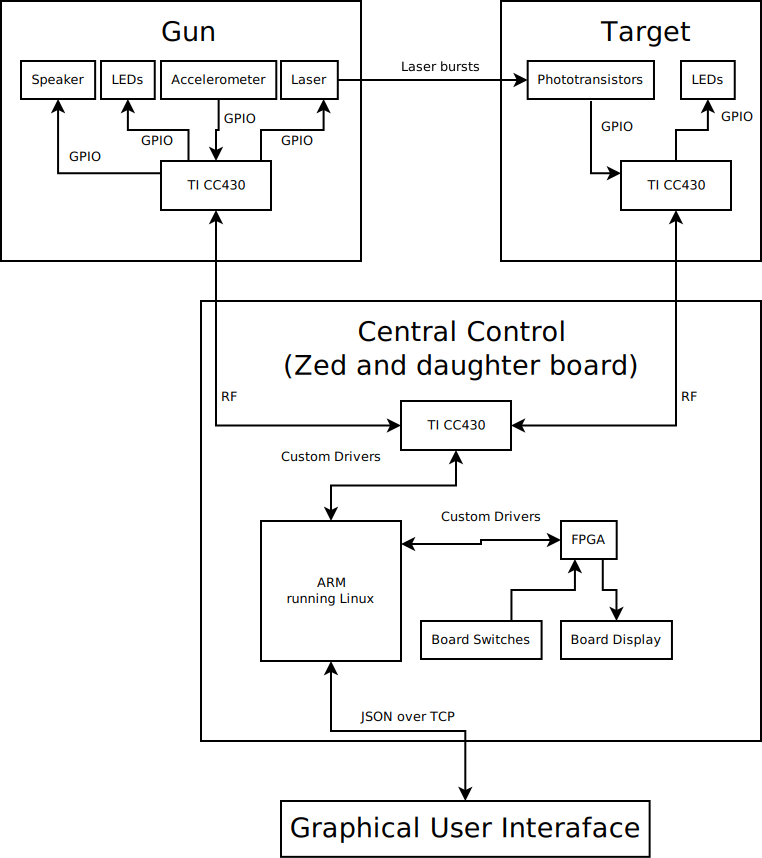
\includegraphics[width=\textwidth, keepaspectratio]{block}

\section{Project Work Schedule}

While dates are fairly set, the amount of hours required is largely a guestimate.
Time measurements will become more accurate as the design is fleshed out and possible implementation issues arise.

\subsection{Hardware}

\begin{tabular}{|l|l|l|r|l|}
\hline
\textbf{Task} & \textbf{Start Date} & \textbf{Completion Date} & \textbf{Days} & \textbf{Assignee} \\
\hline
Order I/O Components for Testing & 2014-02-14 & 2014-02-19 & 4 & Everyone \\
\hline
Final Schematics, BOM, \& Test Plan & 2014-02-15 & 2014-02-28 & 11 & Tyler, Creighton \\
\hline
Initial Component Verification & 2014-02-19 & 2014-02-28 & 8 & Tyler, Creighton \\
\hline
Layout & 2014-03-01 & 2014-01-05 & 4 & Tyler \\
\hline
Place Orders & 2014-03-06 & 2014-03-12 & 5 & TBD \\
\hline
Initial Hardware Assembly \& Testing & 2014-03-24 & 2014-03-30 & 6 & Creighton \\
\hline
Continued Hardware Testing & 2014-03-31 & 2014-04-07 & 6 & James \\
\hline
Build Target Frames & 2014-04-07 & 2014-04-14 & 6 & Tyler \\
\hline
Misc. Fixes & 2014-04-24 & 2014-04-27 & 3 & Everyone \\
\hline
Final Touch-Ups & 2014-04-28 & 2014-05-05 & 6 & Everyone \\
\hline
Final Project Report & 2014-05-06 & 2014-05-09 & 4 & Everyone \\
\hline
\end{tabular}

\subsection{Software}

The software design will take advantage dependency injection to isolate the hardware into interfaces where possible.
This way mock hardware implementations can be used for testing and a large chunk of the software can be developed
independently of the backing hardware.
Software development times include debugging.

\begin{tabular}{|l|l|l|l|l|}
\hline
\textbf{Task} & \textbf{Start Date} & \textbf{Completion Date} & \textbf{Days} & \textbf{Assignee} \\
\hline
Develop JSON UI Protocol & 2014-02-15 & 2014-02-19 & 4 & Matt \\
\hline
Setup TI CC430 Dev Environment & 2014-02-24 & 2014-03-05 & 8 & Matt, James \\
\hline
Develop Game Software (ZedBoard) & 2014-03-06 & 2014-03-30 & 18 & Matt \\
\hline
Develop Gun Software & 2014-03-31 & 2014-04-09 & 8 & Matt \\
\hline
Develop Target Software & 2014-04-09 & 2014-04-18 & 8 & Matt \\
\hline
Develop End-User GUI & 2014-04-14 & 2014-04-23 & 8 & Matt \\
\hline
\end{tabular}

\subsection{Gantt Chart}
\includegraphics[keepaspectratio, angle=90, width=6in]{schedule}

\section{Costs}

Costs are estimates, not hard values.\footnote{Batteries not included}

\subsection{Guns}

\begin{tabular}{|r|l|r|r|}
\hline
\textbf{Qty} & \textbf{Item} & \textbf{Each} & \textbf{Total} \\
\hline
2 & Piezo Buzzer & \$0.79 & \$1.58 \\
\hline
2 & TI CC430 & \$7.00 & \$14.00 \\
\hline
2 & Push-button & \$1.00 & \$2.00 \\
\hline
2 & Accelerometer (BMA222E) & \$3.00 & \$6.00 \\
\hline
2 & Frame (Namco GunCon) & \$12.00 & \$24.00 \\
\hline
\multicolumn{3}{r|}{\textbf{Total:}} & \$47.58 \\
\cline{4-4}
\end{tabular}

The push buttons are for a backup/diagnostic trigger

\subsection{Targets}

\begin{tabular}{|r|l|r|r|}
\hline
\textbf{Qty} & \textbf{Item} & \textbf{Each} & \textbf{Total} \\
\hline
3 & Frame & Max \$5.00 & Max \$15.00 \\
\hline
Max 15 & Tri-color LED & TBD & \$5--10 \\
\hline
12 & Phototransistor & \$0.50 & Max \$6 \\
\hline
3 & TI CC430 & \$7.00 & \$21.00 \\
\hline
3 & Power Supply & \$15.00 & \$45.00 \\
\hline
\multicolumn{3}{r|}{\textbf{Total:}} & \$97.00 \\
\cline{4-4}
\end{tabular}

\subsection{Central Control}

\begin{tabular}{|r|l|r|r|}
\hline
\textbf{Qty} & \textbf{Item} & \textbf{Each} & \textbf{Total} \\
\hline
1 & TI CC430 & \$7.00 & \$21.00 \\
\hline
2 & PCB & \$33.00 & \$66.00 \\
\hline
\multicolumn{3}{r|}{\textbf{Total:}} & \$87.00 \\
\cline{4-4}
\end{tabular}

\subsubsection{Additional Costs}

Allocate an additional \$10.00 for miscellaneous parts (caps, resistors, etc.), bringing us to a total of
roughly \$245.00.

\end{document}
